\section{Configure CMake}

After you have cloned the repository from GitHub, you need to install Qt.

In order to prepare the building process you have to configure CMake either in command prompt or from a GUI CMake program. In Windows as well as in Linux CMake-gui is a GUI CMake program. In \ref{fig:cmakegui_planes} you can see a screenshot of what the cmake program will show after you give it the path to the project (the folder where the main CMakeLists.txt lies) and the folder where you want the project libraries to be built.


\begin{figure}[h]
	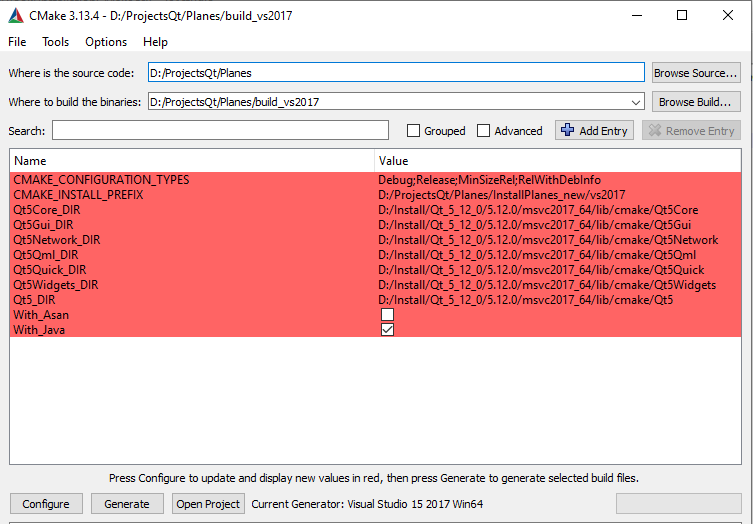
\includegraphics[width = \textwidth]{PlanesCPlusPlus_CMAKE_GUI_Window.png}
	\caption{CMake-GUI Window for project Planes}
	\label{fig:cmakegui_planes}
\end{figure}

You have here several options which need to be set:

\begin{itemize}
	\item CMAKE\_INSTALL\_PREFIX defines the path where the project binaries will be built
	\item Qt*\_DIR are the paths where the various Qt libraries are to be found by the project. Usually you have to define Qt5\_DIR and then the others will be setup automatically.
	\item With\_Asan will activate Address Sanitizer support
	\item With\_Java has to be active when building for the Android application.
\end{itemize}

CMake GUI uses so called generators to define which toolchain is used for compilation. These need to be set for example for Visual Studio (as seen in \ref{fig:cmakegui_planes}), gcc, MinGW or any other toolchain you use to build the project.

Tested binaries of the project used Visual Studio, gcc and MinGW generators.

To perform project configuration click "Configure" and then "Generate".

\section {Binaries}

\subsection{Windows - Visual Studio}

For the Visual Studio generator, after "Generate" is clicked, a solution file is created (.sln). You can use this solution file to open the project. You need to build the INSTALL target inside the project to generate the binaries. 

\subsection {Windows - MinGW} 

You have to choose the MINGW generator before defining the CMAKE variables in the CMAKE-Gui. You have to run Configure and Generate as well as with the Visual Studio generator. After you have done that you have to go to Windows Command Prompt in the build path. There you should give the following command: cmake.exe --build . This will use MinGW's make program to build the program. To install the binaries in the installation path (configured in CMAKE-Gui with CMAKE\_INSTALL\_PREFIX) run cmake.exe --build install .

\subsection {Linux - GCC}

TODO.